\section{Etude de performance et optimisations}\label{sec:part3}
%\paragraph{}Je me suis finalement penché sur les performances de la version 3D de NTMIX développé au cours de ce stage. J'ai dans un premier temps étudié les performances séquentielles du programme (code tel qu'il était à la fin de la première partie) puis les performances de la version parallèle.
\subsection{Présentation du matériel}\label{sec:matos}
L'ensemble des tests suivants ont été réalisés sur les calculateurs internes du Cerfacs, le Bullx B510 et le cluster LENOVO. Ils possèdent les caractéristiques suivantes:

\begin{table}[!ht]
  \begin{center}
    \begin{tabular}{|M{3.5cm}|M{5cm}|M{5cm}|}
      \hline
      & Bullx & Lenovo \\
      \hline
      Noeuds de calcul & 158 & 252 \\
      \hline
      Puissance crête & 53 TFlop/s & 242 TFlop/s \\
      \hline
      Consommation maximale & 51 kW.h & 73 kW.h \\
      \hline
      Consommation à vide & 25 kW.h & 34 kW.h \\
      \hline
      Processeurs & Intel Sandy Bridge bi-socket, 8 coeurs (2.6 GHz) & Intel Haswell bi-socket, 12 coeurs (2.5 GHz) \\
      \hline
      Nb total de coeurs de calculs & 2528 & 6048 \\
      \hline
      Mémoire & 32 Go de mémoire cadencée à 1600 MHz & 64 Go de mémoire cadencée à 2133 MHz \\
      \hline
      Cache L1 & 32 Ko & 32 Ko \\
      \hline
      Cache L2 & 256 Ko & 256 Ko \\
      \hline
      Cache L3 & 20 Mo (partagé) & 30 Mo (partagé) \\
      \hline
      Bande passante inter-noeud & 5 Go/s & 6.4 Go/s \\
      \hline
    \end{tabular}
  \end{center}
  \caption{\label{tab:carac}Caractéristiques des calculateurs du Cerfacs}
\end{table}

\subsection{Métriques utilisées}
\begin{itemize}
\item Le temps passé pour calculer un point, par pas de temps. Cette mesure est exprimée en microsecondes par point par itération ($\mu s/p/it$).

%\item Le nombre d'opérations à virgule flottante par seconde (\textit{Flops: FLoating Point OPeration per Second}). Elle mesure le nombre d'opération par seconde utilisant des nombres réels (ou nombre à virgule flottante). Elle est utile pour vérifier si le code utilise toute la puissance de calcul possible.
\item Scalabilité: la mesure de la scalabilité d'une application permet d'indiquer l'efficacité de celle-ci lorsqu'on augmente le nombre d'éléments parallèle (ici les coeurs). Il existe 2 type de mesure de scalabilité présentées en section \ref{sec:scal}



\end{itemize}




\subsection{Performances séquentielles}
Dans cette partie, on s'intéresse au programme testé et fonctionnel présenté dans la première partie. Avant de commencer à profiler l'application, 3 cas ont été définis; ils permettent de couvrir une plus grande partie du code; en effet chacun de ces cas utilise des parties du code différentes:

\begin{itemize}
\item Cas périodique: le domaine de calcul est périodique, aucun traitement n'est appliqué aux frontières de celui-ci
\item Cas symétrique: les bordures physiques sont traitées avec \textit{NSCBC} 
\item Cas non-périodique: les bordures physiques sont traitées avec \textit{NSCBC} et un schéma décentré est utilisé pour le calcul des gradients aux bordures.
\end{itemize}


Dans chacun des tests, 2 espèces sont présentes. On part d'une taille de 20 points de coté (donc la taille du domaine est de $20\times20\times20$ points) et on l'augmente par pas de 50\%. Pour chacune de ces taille de domaine, on réalise 20 itérations et on calcule la moyenne des temps par points de celles-ci.

%Une fois le programme testé et fonctionnel, j'ai commencé à étudier ses performances. J'ai, dans un premier temps, mesuré un temps de référence pour l'exécution de ce programme; compilation par défaut, donc avec l'option -O2.
\subsubsection{Parcours contigus des tableaux}
Lorsqu'une donnée est utilisée dans le code, elle est copiée en mémoire cache (une mémoire à accès rapide). Suivant le principe de localité spatiale, l'accès à une donnée va probablement être suivie d'un accès à une donnée proche (Ex: parcours de boucle), une ligne de cache est en fait copiée dans la mémoire cache au lieu d'une seule donnée. 
Lorsque qu'on parcourt un tableau dans son ordre de stockage, les données nécessaires sont donc déjà dans le cache, ce qui permet de réduire les coûts de transfert de données. En revanche, si on parcourt un tableau de façon non-contigüe, et que les dimensions de ce tableau sont de tailles conséquentes, un défaut de cache va se produire à chaque itération (la donnée nécessaire n'est pas présente dans le cache et une nouvelle ligne de cache doit être copiée dans le cache), ce qui entraîne un ralentissement de l'application à cause des temps de transfert entre la RAM et le cache.


\paragraph{}Dans les fonctions calculant les gradients, beaucoup de boucles réalisaient des parcours de tableaux non contigus. En Fortran, les tableaux sont stockés en ``row major'' (fig. \ref{fig:rowmajor}); par exemple, les éléments $a_{1,1}$ et $a_{2,1}$ sont à côté en mémoire.

\begin{figure}[ht]
  \centering
  \begin{subfigure}[b]{1\textwidth}
    \centering
    $A_{m,n} = 
    \begin{pmatrix}
      a_{1,1} & a_{1,2} & \cdots & a_{1,n} \\
      a_{2,1} & a_{2,2} & \cdots & a_{2,n} \\
      \vdots  & \vdots  & \ddots & \vdots  \\
      a_{m,1} & a_{m,2} & \cdots & a_{m,n} 
    \end{pmatrix}
    $
  \end{subfigure}
  \vspace{0.6cm}
  
  \begin{subfigure}[b]{1\textwidth}
    \centering
    \begin{tabular}{|c|c|c|c|c|c|c|c|c|c|c|c|c|c|}
      \hline
      %Address & 0 & 1  & & $m-1$ & $m$ & $m+1$ & & $2m-1$ &  & $(n-1)m$ & $(n-1)m+1$ & & $nm-1$ \\
      Address & 0 & 1  & & $m-1$ & $m$ & $m+1$ &  & $nm-1$ \\
      \hline
      Value & $a_{1,1}$ & $a_{2,1}$ & $\cdots$ & $a_{m,1}$ & $a_{1,2}$ & $a_{2,2}$ & $\cdots$ & $a_{m,n}$ \\
      \hline
      \end{tabular}
  \end{subfigure}
  \caption{\label{fig:rowmajor}Stockage des tableaux en Fortran}
\end{figure}


La figure \ref{fig:noncontiguous} montre l'exemple d'une boucle ne parcourant pas un tableau de façon contigüe; en effet, la boucle interne fait varier la seconde dimension le plus vite, or, comme on le voit sur la figure \ref{fig:rowmajor}, les éléments $a_{i,1}$ et $a_{i,2}$ ne sont pas placés à côté en mémoire. On peut donc inverser les 2 boucles pour régler ce problème.


\begin{figure}[!ht]
  \centering
  \begin{lstlisting}[language=Fortran]
    DO JX=3,NX-2
         DO JY=1,NY
            S(JX,JY) = (-U(JX-2,JY)-28.D0*(U(JX-1,JY)-U(JX+1,JY)) &
                        +U(JX+2,JY)) * HX4_INV_X                  &
                        +DELT_SYM_X(JX) * S(JX-1,JY)
         END DO
    END DO
  \end{lstlisting}
  \caption{\label{fig:noncontiguous}Parcours non-contigu}
\end{figure}



\subsubsection{Vectorisation}\label{fig:vecto}
L'application est constituée de nombreuses boucles de calculs parcourant les tableaux contenant les variables conservatives. Il semble donc être un bon candidat pour la vectorisation. La vectorisation est présente sur les processeurs possédant des instructions SIMD (\textit{Single Instruction Multiple Data}). Cela signifie qu'il est possible d'appliquer une opération sur plusieurs éléments à la fois au lieu d'un seul. Comme on peut le voir sur la figure \ref{fig:simd}, si on a une boucle calculant la somme de 2 tableaux; sans vectorisation, le processeur réalisera une addition à la fois, mais avec la vectorisation, il peut traiter les 4 éléments avec une seule instruction, réduisant ainsi le temps de calcul.

\begin{figure}[ht]
  \centering
  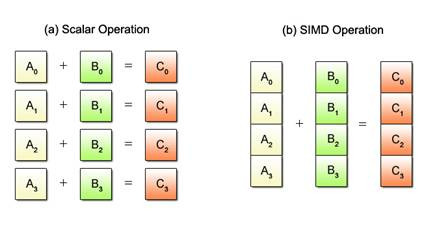
\includegraphics[scale=0.85]{figures/simd.jpg}
  \caption{\label{fig:simd} Instructions SIMD}
\end{figure}


Avant d'activer la vectorisation, des mesures de temps de référence ont été réalisées afin de fournir un temps de comparaison. Les courbes nommées ``Base time'' sur les figures suivantes \ref{fig:bench_scal_nemo} et \ref{fig:bench_scal_neptune} (présentée en annexe \ref{app:seq_neptune}) représentent ce temps de référence (pas de vectorisation mais avec des optimisations automatiques du compilateur).

Sur le cluster LENOVO, le jeu d'instruction AVX2 est disponible, il permet de traiter des vecteurs de 256 bits, soit 4 nombres double précision. Si les boucles réalisent beaucoup de calculs, on peut donc espérer diviser le temps par 4. Sur BULL, c'est le jeu d'instruction AVX qui est disponible; il permet de traiter des vecteurs de 128 bits et le gain maximal potentiel est donc de 2. Cependant, comme on peut le constater sur les figures \ref{fig:bench_scal_nemo} et \ref{fig:bench_scal_neptune}, la vectorisation n'a entraîné qu'un gain d'entre 18 et 25\% selon le cas, indépendamment du jeu d'instruction utilisé. Grâce à Intel Advisor, un logiciel permettant d'analyser la vectorisation réalisée sur les différentes boucles d'une application, il est possible de voir que:
\begin{itemize}
\item certaines fonctions dans lesquelles le programme passe beaucoup de temps ne sont pas vectorisée à cause de dépendances, notamment dans le calculs des gradients. Dans ce cas, on est dépendant de la méthode utilisée pour ces calculs et on ne peut pas forcer la vectorisation des boucles.
\item beaucoup de petites boucles de calcul ne sont pas vectorisées. Ceci est dû à la structure de la mémoire du programme; tous les tableaux contenant des variables conservatives sont en réalité des sous-parties d'un plus grand tableau. Lorsque des opérations sont effectuées sur ces tableaux, le compilateur suppose qu'il travaille sur un unique grand tableau et empêche donc la vectorisation au profit de la cohérence. Pour résoudre ce problème, il suffit d'indiquer au compilateur qu'il n'y a pas aliasing; on garantit ainsi qu'une zone mémoire ne peut être accédée que par un seul nom et que le programme ne dépassera pas les limites d'un tableau. Cependant, comme on peut le voir sur les figures \ref{fig:bench_scal_nemo} et \ref{fig:bench_scal_neptune}, le gain est relativement faible (inférieur à 4\% par rapport aux temps avec la vectorisation seule); 
\end{itemize}



\begin{figure}[!ht]
  \centering
  \begin{subfigure}[b]{0.5\textwidth}
    \centering
    \includegraphics[page=1,scale=0.51]{gnuplot/bench_scalaire_nemo.pdf}
  \caption{\label{fig:bench_scal_nemo_nonper}}
  \end{subfigure}%
  ~
  \begin{subfigure}[b]{0.5\textwidth}
    \centering
    \includegraphics[page=2,scale=0.51]{gnuplot/bench_scalaire_nemo.pdf}
  \caption{\label{fig:bench_scal_nemo_sym}}
  \end{subfigure}
  \begin{subfigure}[b]{0.5\textwidth}
    \centering
    %\includepdf[pages={2}]{gnuplot/bench_scalaire.pdf}
    \includegraphics[page=3,scale=0.51]{gnuplot/bench_scalaire_nemo.pdf}
  \caption{\label{fig:bench_scal_nemo_per}}
  \end{subfigure}
  \caption{\label{fig:bench_scal_nemo}Temps par points des cas tests - LENOVO}
\end{figure}



\begin{figure}[!ht]
  \centering
  \begin{subfigure}[b]{0.5\textwidth}
    \centering
    \includegraphics[scale=0.51]{gnuplot/bench_scalaire_speedup_neptune.pdf}
  \caption{\label{fig:bench_scal_neptune_speedup}}
  \end{subfigure}%
  ~
  \begin{subfigure}[b]{0.5\textwidth}
    \centering
    \includegraphics[scale=0.51]{gnuplot/bench_scalaire_speedup_nemo.pdf}
  \caption{\label{fig:bench_scal_nemo_speedup}}
  \end{subfigure}
  \caption{\label{fig:bench_scal_speedups}Speedup finaux}
\end{figure}

Comme on peut le voir sur les figures \ref{fig:bench_scal_nemo_speedup}, le speedup ($\frac{Base time}{Vectoriztion+alliasing}$) est en constante diminution au fur et à mesure que l'on augmente la taille du domaine. En utilisant \textit{valgrind} avec l'outil \textit{massif} qui permet de profiler l'usage de la mémoire d'un programme, on constate que pour une taille de maillage de $20^3$, environ 27Mo sont utilisés et pour un domaine de 30, environ 48Mo. Seul le cas avec un domaine de taille 20 peut tenir entièrement dans le cache L3 d'un nœud du calculateur Lenovo (cache L3 de 30Mo), tous les cas suivants sont donc fortement dépendant des transferts de données se réalisant depuis la RAM, limitant ainsi le speedup obtenu grâce à la vectorisation.

\subsubsection{Alignement de la mémoire}
Lorsqu'on vectorise un code, il est conseillé d'aligner la mémoire afin d'
Cependant, les tableaux se trouvant dans les modules ne peuvent être aligné



\subsection{Performances parallèle}


\subsubsection{Méthode de communication}
Cette section traite des méthodes utilisées pour réaliser les communication entre les processus pour échanger les zones d'overlapping.

%Avant de comparer les méthodes de recouvrement, je me suis dans un premier temps interréssé aux méthodes de communication utilisées pour la première méthode (\ref{sec:}). Pour cela, j'ai comparer la durée passée dans des communications pour chacune des méthode et ceux pour différentes taille de grille.


%mesurer le temps d'exécution par point par pas de temps de chacune des méthodes pour différentes taille de grille.


%\subsubsection{Méthode de recouvrement}
%Je compare ici les 2 méthodes utilisée pour le recouvrement de domain présentées dans la partie précedente. Pour rappel: 



%\subsubsection{Décomposition du domaine}
%Le découpage du domaine est entièrement configurable par l'utilisateur, nous verons donc ici l'influence que ce découpage peut avoir sur le temps d'exécution du programme. 

%https://www.sharcnet.ca/help/index.php/Measuring_Parallel_Scaling_Performance
\subsection{Scalabilité}\label{sec:scal}

\subsubsection{Scalabilité forte}\label{sec:scal-strong}
Pour une taille de problème fixée, on augmente le nombre de processus. Dans le cas d'une application réalisant beaucoup de calculs, le but est de trouver le point auquel on obtient un temps d'exécution raisonnable mais en limitant les surcoût induit par un programme parallèle.

$$E=\frac{t_1}{n\times t_n}$$ avec $t_i$ le temps d'exécution avec $i$ processus et $t_1$ le temps d'exécution avec un seul processus.

\paragraph{}On recherche donc une taille de problème la plus grande possible afin de pouvoir augmenter le nombre de processus. Pour cela, il faut trouver une taille de problème qui occupe le plus de mémoire possible sur un noeud. J'ai utilisée MPS pour mesurer la mémoire totale utilisée par tous les processus MPI sur un noeud. On trouve que pour un domaine de $400^3$ points de maillage, la mémoire utilisée est d'environ 55Go. La mémoire disponible sur un noeud du cluster LENOVO est de 64Go donc cette taille de domaine sera utilisée pour mesurer la scalabilité forte de l'application.

\subsubsection{Scalabilité faible}\label{sec:scal-weak}
Dans ce cas, la taille du problème assignée à chaque processus reste constante et on ajoute des processeurs dans le but d'augmenter la taille globale du problème. Étant donné que le pattern de communication ne change pas (chaque processus communique avec ses voisins directs), le but est de mettre en évidence le coût des communications globales (ici les reduce pour le calcul du pas de temps maximal).


$$E=\frac{t_1}{t_i}$$ avec $t_i$ le temps d'exécution avec $i$ processus.


%http://citeseerx.ist.psu.edu/viewdoc/download;jsessionid=D9B131203AACF6CB76730F3678DE81ED?doi=10.1.1.49.3513&rep=rep1&type=pdf


%https://books.google.fr/books?hl=en&lr=&id=bsrkrw5MdtUC&oi=fnd&pg=PP2&dq=Numerical+computation+of+internal+and+external+flows&ots=a4zO-j_pzd&sig=2MOJYmYvrd2Tq55eL6ZsU3bmyoE&redir_esc=y#v=onepage&q=Numerical%20computation%20of%20internal%20and%20external%20flows&f=false
